\documentclass[border=5pt]{standalone}
\usepackage[T1]{fontenc}
\usepackage{lmodern}
\usepackage{pgfplots}
\usepgfplotslibrary{groupplots}
\pgfplotsset{compat=1.18}
\begin{document}
\sffamily
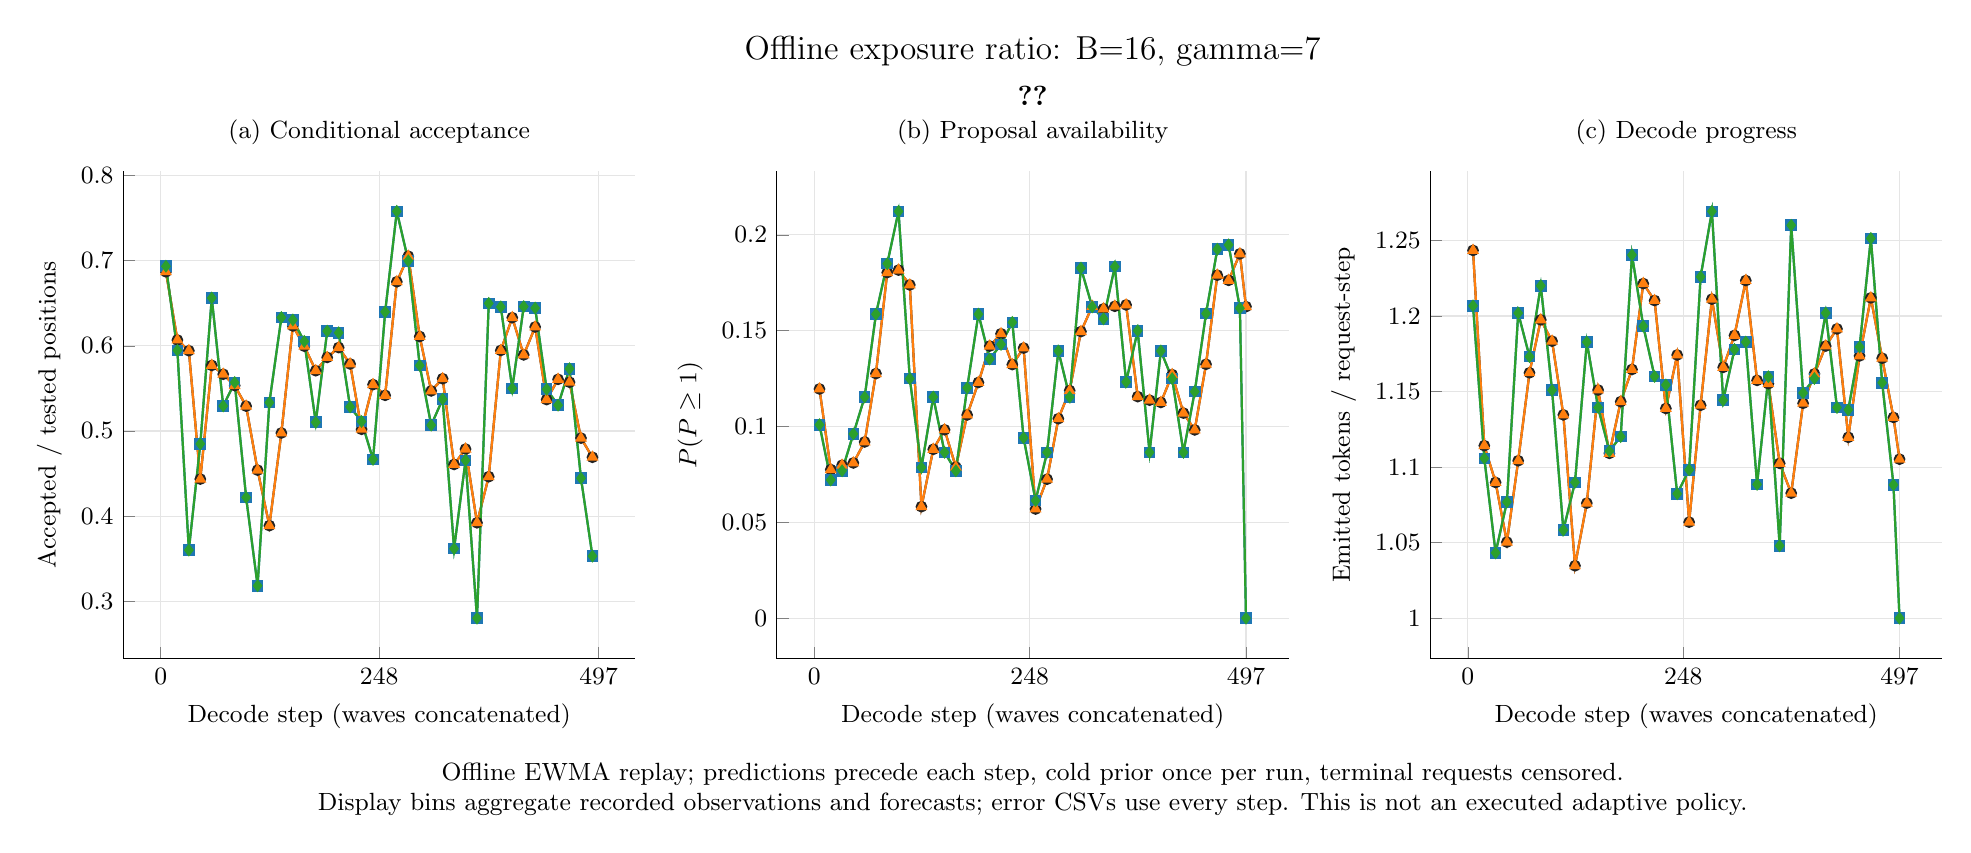
\begin{tikzpicture}
\definecolor{series0}{HTML}{222222}
\definecolor{series1}{HTML}{1f77b4}
\definecolor{series2}{HTML}{ff7f0e}
\definecolor{series3}{HTML}{2ca02c}
\definecolor{series4}{HTML}{d62728}
\definecolor{series5}{HTML}{9467bd}
\definecolor{series6}{HTML}{8c564b}
\definecolor{series7}{HTML}{e377c2}
\begin{groupplot}[group style={group size=3 by 1,horizontal sep=1.8cm},width=6.5cm,height=6.2cm,scale only axis,grid=major,grid style={gray!20},axis lines*=left,tick label style={font=\small},label style={font=\small},title style={font=\small},unbounded coords=jump]
\nextgroupplot[title={(a) Conditional acceptance},xlabel={Decode step (waves concatenated)},ylabel={Accepted / tested positions},xtick={0,248,497},xticklabels={0,248,497},scaled y ticks=false,yticklabel style={/pgf/number format/fixed,/pgf/number format/precision=2},legend columns=4,legend to name=sharedlegend,legend style={draw=none,font=\small,/tikz/every even column/.append style={column sep=8pt}}]
\addplot+[color=series0,mark=*,mark size=1.7pt,mark options={fill=series0,draw=series0},line width=0.8pt] coordinates {(6,0.687072186869) (19,0.606892670672) (32,0.594324012978) (45,0.443472929689) (58,0.577046263215) (71,0.566689698488) (84,0.553333480705) (97,0.529208552734) (110,0.453997681179) (123.38461538461539,0.388766806699) (137,0.497631248941) (150,0.623463091211) (163,0.599669624501) (176,0.570824099455) (189,0.586419886261) (202,0.597986335847) (215,0.578792164587) (228,0.501978680529) (241,0.55452822799) (254.76923076923077,0.54190234943) (268,0.675341361572) (281,0.705362205828) (294,0.611014768514) (307,0.547082400571) (320,0.561411223895) (333,0.460664031795) (346,0.478758880891) (359,0.392127482276) (372.3076923076923,0.446263169776) (386,0.59465704138) (399,0.633193279862) (412,0.589423369184) (425,0.622215292812) (438,0.536902215785) (451,0.560690090111) (464,0.557289992404) (477,0.491618444133) (490,0.469084638718) (497,nan)};
\addlegendentry{run 0: forecast}
\addplot+[only marks,forget plot,color=series0,mark=o,mark size=2.1pt,mark options={fill=white,line width=0.45pt}] coordinates {};
\addplot+[color=series1,mark=square*,mark size=1.7pt,mark options={fill=series1,draw=series1},line width=0.8pt] coordinates {(6,0.693548387097) (19,0.594594594595) (32,0.36) (45,0.484848484848) (58,0.65625) (71,0.529411764706) (84,0.556962025316) (97,0.421875) (110,0.318181818182) (123.38461538461539,0.533333333333) (137,0.633333333333) (150,0.630434782609) (163,0.605263157895) (176,0.510204081633) (189,0.617283950617) (202,0.615384615385) (215,0.528301886792) (228,0.511111111111) (241,0.466666666667) (254.76923076923077,0.64) (268,0.758064516129) (281,0.7) (294,0.576923076923) (307,0.506849315068) (320,0.537313432836) (333,0.36170212766) (346,0.465517241379) (359,0.28) (372.3076923076923,0.65) (386,0.645833333333) (399,0.55) (412,0.646153846154) (425,0.644444444444) (438,0.549019607843) (451,0.530303030303) (464,0.573170731707) (477,0.444444444444) (490,0.352941176471) (497,nan)};
\addlegendentry{run 0: observed}
\addplot+[only marks,forget plot,color=series1,mark=o,mark size=2.1pt,mark options={fill=white,line width=0.45pt}] coordinates {};
\addplot+[color=series2,mark=triangle*,mark size=1.7pt,mark options={fill=series2,draw=series2},line width=0.8pt] coordinates {(6,0.687072186869) (19,0.606892670672) (32,0.594324012978) (45,0.443472929689) (58,0.577046263215) (71,0.566689698488) (84,0.553333480705) (97,0.529208552734) (110,0.453997681179) (123.38461538461539,0.388766806699) (137,0.497631248941) (150,0.623463091211) (163,0.599669624501) (176,0.570824099455) (189,0.586419886261) (202,0.597986335847) (215,0.578792164587) (228,0.501978680529) (241,0.55452822799) (254.76923076923077,0.54190234943) (268,0.675341361572) (281,0.705362205828) (294,0.611014768514) (307,0.547082400571) (320,0.561411223895) (333,0.460664031795) (346,0.478758880891) (359,0.392127482276) (372.3076923076923,0.446263169776) (386,0.59465704138) (399,0.633193279862) (412,0.589423369184) (425,0.622215292812) (438,0.536902215785) (451,0.560690090111) (464,0.557289992404) (477,0.491618444133) (490,0.469084638718) (497,nan)};
\addlegendentry{run 1: forecast}
\addplot+[only marks,forget plot,color=series2,mark=o,mark size=2.1pt,mark options={fill=white,line width=0.45pt}] coordinates {};
\addplot+[color=series3,mark=diamond*,mark size=1.7pt,mark options={fill=series3,draw=series3},line width=0.8pt] coordinates {(6,0.693548387097) (19,0.594594594595) (32,0.36) (45,0.484848484848) (58,0.65625) (71,0.529411764706) (84,0.556962025316) (97,0.421875) (110,0.318181818182) (123.38461538461539,0.533333333333) (137,0.633333333333) (150,0.630434782609) (163,0.605263157895) (176,0.510204081633) (189,0.617283950617) (202,0.615384615385) (215,0.528301886792) (228,0.511111111111) (241,0.466666666667) (254.76923076923077,0.64) (268,0.758064516129) (281,0.7) (294,0.576923076923) (307,0.506849315068) (320,0.537313432836) (333,0.36170212766) (346,0.465517241379) (359,0.28) (372.3076923076923,0.65) (386,0.645833333333) (399,0.55) (412,0.646153846154) (425,0.644444444444) (438,0.549019607843) (451,0.530303030303) (464,0.573170731707) (477,0.444444444444) (490,0.352941176471) (497,nan)};
\addlegendentry{run 1: observed}
\addplot+[only marks,forget plot,color=series3,mark=o,mark size=2.1pt,mark options={fill=white,line width=0.45pt}] coordinates {};
\nextgroupplot[title={(b) Proposal availability},xlabel={Decode step (waves concatenated)},ylabel={$P(P \geq 1)$},xtick={0,248,497},xticklabels={0,248,497},scaled y ticks=false,yticklabel style={/pgf/number format/fixed,/pgf/number format/precision=2}]
\addplot+[color=series0,mark=*,mark size=1.7pt,mark options={fill=series0,draw=series0},line width=0.8pt] coordinates {(6,0.119618064667) (19,0.0775520814192) (32,0.0798147837624) (45,0.081012497356) (58,0.0919553211616) (71,0.127638168951) (84,0.180351407247) (97,0.181655349844) (110,0.173897041036) (123.38461538461539,0.058195809994) (137,0.0881223156451) (150,0.098318386125) (163,0.0788511125555) (176,0.106049827988) (189,0.123013187195) (202,0.142005957033) (215,0.148421261626) (228,0.1323473535) (241,0.140980376234) (254.76923076923077,0.0569727389797) (268,0.0725271487186) (281,0.104102070025) (294,0.118777582252) (307,0.149559201426) (320,0.162748824412) (333,0.161430009641) (346,0.162764541465) (359,0.163486539426) (372.3076923076923,0.115627789829) (386,0.1137619798) (399,0.112573155582) (412,0.12710100946) (425,0.107026005278) (438,0.0982409830238) (451,0.132508039462) (464,0.178993816568) (477,0.176308166034) (490,0.190141026403) (497,0.162574820217)};
\addplot+[only marks,forget plot,color=series0,mark=o,mark size=2.1pt,mark options={fill=white,line width=0.45pt}] coordinates {};
\addplot+[color=series1,mark=square*,mark size=1.7pt,mark options={fill=series1,draw=series1},line width=0.8pt] coordinates {(6,0.100961538462) (19,0.0721153846154) (32,0.0769230769231) (45,0.0961538461538) (58,0.115384615385) (71,0.158653846154) (84,0.185) (97,0.212290502793) (110,0.125) (123.38461538461539,0.0786516853933) (137,0.115384615385) (150,0.0865384615385) (163,0.0769230769231) (176,0.120192307692) (189,0.158653846154) (202,0.135265700483) (215,0.142857142857) (228,0.154362416107) (241,0.0941176470588) (254.76923076923077,0.0613496932515) (268,0.0865384615385) (281,0.139423076923) (294,0.115384615385) (307,0.182692307692) (320,0.162436548223) (333,0.15625) (346,0.183431952663) (359,0.123287671233) (372.3076923076923,0.15) (386,0.0865384615385) (399,0.139423076923) (412,0.125) (425,0.0865384615385) (438,0.118226600985) (451,0.158974358974) (464,0.192513368984) (477,0.194805194805) (490,0.161764705882) (497,0)};
\addplot+[only marks,forget plot,color=series1,mark=o,mark size=2.1pt,mark options={fill=white,line width=0.45pt}] coordinates {};
\addplot+[color=series2,mark=triangle*,mark size=1.7pt,mark options={fill=series2,draw=series2},line width=0.8pt] coordinates {(6,0.119618064667) (19,0.0775520814192) (32,0.0798147837624) (45,0.081012497356) (58,0.0919553211616) (71,0.127638168951) (84,0.180351407247) (97,0.181655349844) (110,0.173897041036) (123.38461538461539,0.058195809994) (137,0.0881223156451) (150,0.098318386125) (163,0.0788511125555) (176,0.106049827988) (189,0.123013187195) (202,0.142005957033) (215,0.148421261626) (228,0.1323473535) (241,0.140980376234) (254.76923076923077,0.0569727389797) (268,0.0725271487186) (281,0.104102070025) (294,0.118777582252) (307,0.149559201426) (320,0.162748824412) (333,0.161430009641) (346,0.162764541465) (359,0.163486539426) (372.3076923076923,0.115627789829) (386,0.1137619798) (399,0.112573155582) (412,0.12710100946) (425,0.107026005278) (438,0.0982409830238) (451,0.132508039462) (464,0.178993816568) (477,0.176308166034) (490,0.190141026403) (497,0.162574820217)};
\addplot+[only marks,forget plot,color=series2,mark=o,mark size=2.1pt,mark options={fill=white,line width=0.45pt}] coordinates {};
\addplot+[color=series3,mark=diamond*,mark size=1.7pt,mark options={fill=series3,draw=series3},line width=0.8pt] coordinates {(6,0.100961538462) (19,0.0721153846154) (32,0.0769230769231) (45,0.0961538461538) (58,0.115384615385) (71,0.158653846154) (84,0.185) (97,0.212290502793) (110,0.125) (123.38461538461539,0.0786516853933) (137,0.115384615385) (150,0.0865384615385) (163,0.0769230769231) (176,0.120192307692) (189,0.158653846154) (202,0.135265700483) (215,0.142857142857) (228,0.154362416107) (241,0.0941176470588) (254.76923076923077,0.0613496932515) (268,0.0865384615385) (281,0.139423076923) (294,0.115384615385) (307,0.182692307692) (320,0.162436548223) (333,0.15625) (346,0.183431952663) (359,0.123287671233) (372.3076923076923,0.15) (386,0.0865384615385) (399,0.139423076923) (412,0.125) (425,0.0865384615385) (438,0.118226600985) (451,0.158974358974) (464,0.192513368984) (477,0.194805194805) (490,0.161764705882) (497,0)};
\addplot+[only marks,forget plot,color=series3,mark=o,mark size=2.1pt,mark options={fill=white,line width=0.45pt}] coordinates {};
\nextgroupplot[title={(c) Decode progress},xlabel={Decode step (waves concatenated)},ylabel={Emitted tokens / request-step},xtick={0,248,497},xticklabels={0,248,497},scaled y ticks=false,yticklabel style={/pgf/number format/fixed,/pgf/number format/precision=2}]
\addplot+[color=series0,mark=*,mark size=1.7pt,mark options={fill=series0,draw=series0},line width=0.8pt] coordinates {(6,1.2434009221) (19,1.11418132404) (32,1.08983062207) (45,1.05036123941) (58,1.10419541114) (71,1.16240313126) (84,1.197459142) (97,1.18333783756) (110,1.1345538151) (123.38461538461539,1.03469035513) (137,1.0761585805) (150,1.15101953116) (163,1.10910686272) (176,1.14329842023) (189,1.16460829322) (202,1.22146190327) (215,1.21022080369) (228,1.1387888398) (241,1.17420510425) (254.76923076923077,1.06356870701) (268,1.14092508757) (281,1.211135884) (294,1.16600836035) (307,1.18715360009) (320,1.22345058877) (333,1.15738410106) (346,1.15518109966) (359,1.10247609833) (372.3076923076923,1.08273875784) (386,1.14224182372) (399,1.16168218382) (412,1.18010976827) (425,1.19146225132) (438,1.11969902974) (451,1.17358305823) (464,1.21199463862) (477,1.1720473294) (490,1.13287590525) (497,1.10523040035)};
\addplot+[only marks,forget plot,color=series0,mark=o,mark size=2.1pt,mark options={fill=white,line width=0.45pt}] coordinates {};
\addplot+[color=series1,mark=square*,mark size=1.7pt,mark options={fill=series1,draw=series1},line width=0.8pt] coordinates {(6,1.20673076923) (19,1.10576923077) (32,1.04326923077) (45,1.07692307692) (58,1.20192307692) (71,1.17307692308) (84,1.22) (97,1.15083798883) (110,1.05833333333) (123.38461538461539,1.08988764045) (137,1.18269230769) (150,1.13942307692) (163,1.11057692308) (176,1.12019230769) (189,1.24038461538) (202,1.19323671498) (215,1.16) (228,1.15436241611) (241,1.08235294118) (254.76923076923077,1.0981595092) (268,1.22596153846) (281,1.26923076923) (294,1.14423076923) (307,1.17788461538) (320,1.18274111675) (333,1.08854166667) (346,1.15976331361) (359,1.04794520548) (372.3076923076923,1.26) (386,1.14903846154) (399,1.15865384615) (412,1.20192307692) (425,1.13942307692) (438,1.13793103448) (451,1.17948717949) (464,1.2513368984) (477,1.15584415584) (490,1.08823529412) (497,1)};
\addplot+[only marks,forget plot,color=series1,mark=o,mark size=2.1pt,mark options={fill=white,line width=0.45pt}] coordinates {};
\addplot+[color=series2,mark=triangle*,mark size=1.7pt,mark options={fill=series2,draw=series2},line width=0.8pt] coordinates {(6,1.2434009221) (19,1.11418132404) (32,1.08983062207) (45,1.05036123941) (58,1.10419541114) (71,1.16240313126) (84,1.197459142) (97,1.18333783756) (110,1.1345538151) (123.38461538461539,1.03469035513) (137,1.0761585805) (150,1.15101953116) (163,1.10910686272) (176,1.14329842023) (189,1.16460829322) (202,1.22146190327) (215,1.21022080369) (228,1.1387888398) (241,1.17420510425) (254.76923076923077,1.06356870701) (268,1.14092508757) (281,1.211135884) (294,1.16600836035) (307,1.18715360009) (320,1.22345058877) (333,1.15738410106) (346,1.15518109966) (359,1.10247609833) (372.3076923076923,1.08273875784) (386,1.14224182372) (399,1.16168218382) (412,1.18010976827) (425,1.19146225132) (438,1.11969902974) (451,1.17358305823) (464,1.21199463862) (477,1.1720473294) (490,1.13287590525) (497,1.10523040035)};
\addplot+[only marks,forget plot,color=series2,mark=o,mark size=2.1pt,mark options={fill=white,line width=0.45pt}] coordinates {};
\addplot+[color=series3,mark=diamond*,mark size=1.7pt,mark options={fill=series3,draw=series3},line width=0.8pt] coordinates {(6,1.20673076923) (19,1.10576923077) (32,1.04326923077) (45,1.07692307692) (58,1.20192307692) (71,1.17307692308) (84,1.22) (97,1.15083798883) (110,1.05833333333) (123.38461538461539,1.08988764045) (137,1.18269230769) (150,1.13942307692) (163,1.11057692308) (176,1.12019230769) (189,1.24038461538) (202,1.19323671498) (215,1.16) (228,1.15436241611) (241,1.08235294118) (254.76923076923077,1.0981595092) (268,1.22596153846) (281,1.26923076923) (294,1.14423076923) (307,1.17788461538) (320,1.18274111675) (333,1.08854166667) (346,1.15976331361) (359,1.04794520548) (372.3076923076923,1.26) (386,1.14903846154) (399,1.15865384615) (412,1.20192307692) (425,1.13942307692) (438,1.13793103448) (451,1.17948717949) (464,1.2513368984) (477,1.15584415584) (490,1.08823529412) (497,1)};
\addplot+[only marks,forget plot,color=series3,mark=o,mark size=2.1pt,mark options={fill=white,line width=0.45pt}] coordinates {};
\end{groupplot}
\path (group c1r1.north west) -- node[above=1.2cm,font=\large] {Offline exposure ratio: B=16, gamma=7} (group c3r1.north east);
\path (group c1r1.north west) -- node[above=0.7cm] {\ref{sharedlegend}} (group c3r1.north east);
\path (group c1r1.south west) -- node[below=1.2cm,align=center,font=\small] {Offline EWMA replay; predictions precede each step, cold prior once per run, terminal requests censored.\\Display bins aggregate recorded observations and forecasts; error CSVs use every step. This is not an executed adaptive policy.} (group c3r1.south east);
\end{tikzpicture}
\end{document}
